\documentclass[11pt]{article}
\usepackage[margin=1in]{geometry}
\usepackage{setspace}
\usepackage{iftex}
\usepackage{amsmath,amssymb}
\usepackage{graphicx}

\ifPDFTeX
  \usepackage[T1]{fontenc}
  \usepackage{newtxtext,newtxmath}
\else
  \usepackage{fontspec}
  \setmainfont{Times New Roman}
\fi

\setstretch{1.0}
\setlength{\parskip}{0.4em}
\setlength{\parindent}{0pt}
\pagenumbering{gobble}

\begin{document}

\begin{titlepage}
\centering
\vspace*{1in}
{\LARGE \textbf{Harnessing the Generative Quantum Eigensolver for Next-Generation Materials Design} \par}
\vspace{0.35in}
{\large \textit{Global Industry Challenge (GIC) 2026} \par}
\vspace{0.5in}
{\large Date: \today \par}
\vspace{0.3in}
\centering
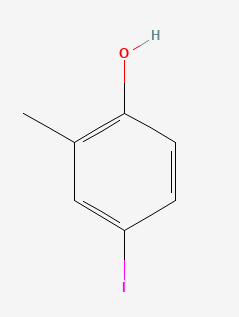
\includegraphics[width=0.35\textwidth]{../img/4-Iodo-2-methylphenol.png}
\vspace{0.25em}

{\footnotesize Figure 1: 4-Iodo-2-methylphenol (IMePh) structure. Source: PubChem.\par}
\vfill
{\large \textbf{Team Name} \par}
\vspace{0.25in}
\begin{tabular}{lll}
Name & Profession & Email \\
\hline
Niraj Venkat & Student and Researcher & Email \\
Something & Some Profession & Email \\
\end{tabular}
\vspace*{0.6in}
\end{titlepage}

\noindent\textbf{Strategic Context}\\
This Phase 1 concept addresses the core quantum-simulation bottleneck in EUV photoresist design: predicting the photoabsorption spectrum and the downstream electron-emission pathways that control lithographic blur. The solution is designed for utility-scale fault-tolerant quantum computers (FTQCs), not near-term NISQ devices, because the relevant observables require deeper circuits, richer excited-state structure, and more stable error budgets than can be expected from shallow prototypes. The goal is to keep the workflow implementation-ready while still framed at the level of a Phase 1 technical overview.

\noindent\textbf{Proposed Solution Architecture}\\
We propose a hybrid quantum-classical architecture centered on a Generative Quantum Eigensolver (GQE)-style search process. A generative model proposes compact circuit structures, and a hybrid training loop ranks them against target energy and transition metrics for a representative molecular target such as 4-Iodo-2-methylphenol. This architecture is intended to prioritize circuit families that can recover the EUV photoabsorption spectrum, low-lying excited states, and transition observables while remaining systematic enough to extend across chemically related molecules through materials-informatics transfer.

\noindent\textbf{Quantum Modeling Workflow}\\
The modeling workflow captures the key photophysical chain at a technical but not overly granular level: absorption of a 92 eV photon, attosecond photoionization, formation of a core-ionized state, femtosecond Auger decay, and the generation of primary, Auger, and secondary electrons. Those secondary electrons undergo inelastic scattering in the resist matrix and drive the chemistry that ultimately produces radiation-induced blur and line-edge roughness. Hamiltonians are constructed for candidate molecules, evaluated through differentiable quantum circuits, and updated as molecular geometry or active-space assumptions evolve. Results are organized for a materials-informatics handoff that ranks candidates by their predicted spectral and electron-emission behavior.

We model each candidate with a second-quantized electronic Hamiltonian,
\begin{equation}
\hat{H} = E_{\mathrm{core}} + \sum_{pq\sigma} h_{pq}\, a^{\dagger}_{p\sigma} a_{q\sigma}
+ \frac{1}{2}\sum_{pqrs\sigma\tau} g_{pqrs}\, a^{\dagger}_{p\sigma} a_{q\sigma} a^{\dagger}_{r\tau} a_{s\tau},
\end{equation}
then map to qubits using Jordan--Wigner so that \(\hat{H}=\sum_{\ell} c_{\ell} P_{\ell}\) with Pauli strings \(P_{\ell}\). The GQE policy samples an operator sequence from a learned pool,
\begin{equation}
\rho(\mathbf{j}) = U_{j_L}\cdots U_{j_1}\,\rho_0\,U_{j_1}^{\dagger}\cdots U_{j_L}^{\dagger},
\qquad
E(\mathbf{j}) = \mathrm{Tr}\!\left[\hat{H}\rho(\mathbf{j})\right],
\end{equation}
and optimizes a sequence-level objective that biases lower-energy circuits,
\begin{equation}
\mathcal{L}_{\mathrm{GQE}} = \left(\sum_{i=1}^{L} w_{j_i} - E(\mathbf{j})\right)^2.
\end{equation}
For spectroscopy we estimate transition observables through the dipole response,
\begin{equation}
\sigma(\omega) \propto \omega\sum_{F\neq I}\sum_{\rho\in\{x,y,z\}}
\frac{|\langle F|\hat{\mu}_{\rho}|I\rangle|^2\,\eta}{(E_F-E_I-\omega)^2+\eta^2},
\end{equation}
which enables direct comparison to classical XAS reference spectra.

\noindent\textbf{Technical Stack and Implementation Path}\\
PennyLane is the quantum programming framework for implementation. We will use PennyLane to build Hamiltonians from electronic-structure inputs, define differentiable quantum circuits, manage shot budgets, and run device-agnostic experiments across simulators and FTQC-oriented backends with mitigation hooks for noisy execution. The GQE workflow uses a classical generative model to propose ansatz sequences, then ranks them using measured observables and hybrid optimization. This provides a clean path from the example notebooks to a reproducible pipeline that can later be extended from a single target molecule to a small family of EUV-relevant compounds.

\noindent\textbf{Expected Phase 1 Deliverable and Validation}\\
Phase 1 delivers a reproducible prototype that computes a prioritized set of quantum-derived metrics for 4-iodo-2-methylphenol (IMePh) and a small set of related molecules, then returns a ranked candidate list for further study. Validation will compare key energies and transition observables against trusted classical references on tractable active spaces and assess whether the hybrid workflow preserves ranking quality while improving iteration speed\footnote{Primary implementation reference: K. Keithley et al., \"Auger Spectroscopy via Generative Quantum Eigensolver: A Quantum Approach to Molecular Excitations,\" arXiv:2603.12859v1 (2026), https://arxiv.org/abs/2603.12859v1.}. The emphasis is feasibility, reproducibility, and decision utility rather than full-spectrum photochemistry coverage.

\noindent\textbf{Conclusion}\\
This proposal establishes a pragmatic path from high-level concept to executable code by coupling GQE-style search with a PennyLane-based hybrid stack that is explicitly aligned to FTQC-scale requirements. The result is a coherent Phase 1 foundation for scalable quantum-enabled materials discovery: technically credible, implementation-oriented, and structured to hand off cleanly into future materials-informatics and photoresist-design workflows.

\end{document}
